\chapter{Increasing ABM Integration}
\label{chap:land}

\newcommand{\NSE}[1]{\text{NSE}_{\text{#1}}}

% The last chapter was about the agricultural land-use ABM
% This chapter is going to be about the land-cover transition ABM
% This model also uses deep reinforcement learning in order to train agents
% The goal of this model is to demonstrate the predictive accuracy of the model
% and to prove the viability of the methodology, that being,
% that adding learning to an ABM allows for more meaningful decision-making
% AND that the ABM part allows the learning to capture features that
% might be hard to model otherwise

The previous chapter demonstrated how an agent-based model can be
implemented with machine learning in order to induce a model of
individual behavior.
This chapter will go on to show how adding a transfer learning
calibration step, in cases where there exists some external metric
for determining the ABM's performance as a result of agent behavior,
can be integrated into this kind of ABM in order to adjust
agent training in a way that increases model performance.
This method is applied in the creation of a land-cover transition
model of a study area in the Lake Champlain Basin of Vermont.

\section{Methodology}
\label{sec:land_methods}
\label{sec:land_cal}

The methodology used here is similar to the methodology presented in
Chapter~\ref{chap:farm}, with the addition of an external
calibration step that takes place during model training.
Because there is an external method for validating the
output of the model for each training episode,
a traditional learning step can be incorporated into the
transfer learning step as a form of adaptive transfer learning,
where there base transfer rate~$\tau$ in
the transfer learning update (Eq~\ref{eq:tr})
is replaced with an adjusted transfer rate~$\tau_{adj}$
as in Equation~\ref{eq:tra}.

\begin{equation}
\label{eq:tra}
\forall\theta'_i\in\Theta'\left[
\theta'_i\leftarrow\tau_{adj}+(1-\tau_{adj})\theta'_i
\right]
\end{equation}

For a given calibration method, that is, a loss function
for overall model performance, the adjusted transfer rate
can be set for each transfer update based on the performance
of the model in each transfer episode.
This allows transfer episodes with a higher metric of model
performance to have a greater impact on the weights of the
target network architecture, whereas transfer episodes that
demonstrated poorer performance would have a lesser impact
on the target architecture.

\section{Experimental Design}
\label{sec:land_exp}

\subsection{Model Overview}

In order to test this calibration methodology and an
increased degree of integration of deep machine learning
techniques into agent-based modeling, a second experimental
ABM was developed.
This ABM is also a model of a study area within the Lake~Champlain
Basin of Vermont, but expanded to included systems outside
of the agricultural sector, as forestry and urban commercial
and residential systems are also included.
In this model, agent decision-making not only impacts their
economic state, but also impacts how the land-cover of the
land associated with each agent develops and changes over time.
The land-cover change is modeled as the stochastic byproduct
of agent action, wherein, for example, an agricultural agent
deciding to increase its productivity with regard to grazing
animals may result in an increase in its beef 
production factor~$p_b$ or a conversion of some unused forested 
land cells on the agent's property into in-use pasture land
cells.

Unlike the model described in Chapter~\ref{chap:farm},
the individual behavior of agents in this model is not its
primary area of interest.
Because real-world data exists for land-cover,
there exists an external, objective method for determining
the accuracy of model performance within a training episode.
The goal of this model is to explore the potential of using
real-world land-cover data and the calibration step 
and its adjustments to learning~transfer to steer agent learning, 
and consequently decision-making, in the direction of an overall 
increase in the predictive accuracy of the model.



\subsubsection{Representing Land Cover}

Real world land cover data for the study area was taken
for the United States Geological Survey's National Land Cover Dataset (NLCD)
for four years: 2001, 2006, 2011, and 2016.
This dataset divides the study area into a matrix of 30m by 30m
land cells which have been assigned one of 15 NLCD land cover classes.
For the purposes of this model, these 15 classes were divided into
6 cover categories: urban, forested, agricultural, barren, grassland/scrub,
and other.
These categories and their corresponding NLCD land cover classes
are listed in Table~\ref{tab:nlcd}.
A plot of the NLCD representation of the study area for NLCD year 2001
is shown in Figure~\ref{fig:land_plot}.

%% TAB: NLCD ---------------------------------------------------------------
\begin{table}
\centering
\caption{A listing of the 15 NLCD cover classes that are present in
the dataset for the study area, their NLCD encoding,
and their associated cover category within the model.}
\label{tab:nlcd}
\begin{tabular}{llc}
\hline
\hline
    Cover Category & NLCD Cover Class & NLCD Encoding \\
\hline
    Urban & Open Space Urban & 21 \\
    & Low Density Urban & 22 \\
    & Medium Density Urban & 23 \\
    & High Density Urban & 24 \\
    Forested & Deciduous Forest & 41 \\
    & Evergreen Forest & 42 \\
    & Mixed Forest & 43 \\
    Agricultural 
    & Pasture & 81 \\
    & Crops & 82\\
    Barren & Barren & 31 \\
    Grassland/Scrub & Scrub & 52 \\
    & Grassland & 71 \\
    Other & Water & 11 \\
    & Wetlands Woody & 90 \\
    & Wetlands Other & 95 \\
\hline
\end{tabular}
\end{table}

\begin{figure}
\centering
    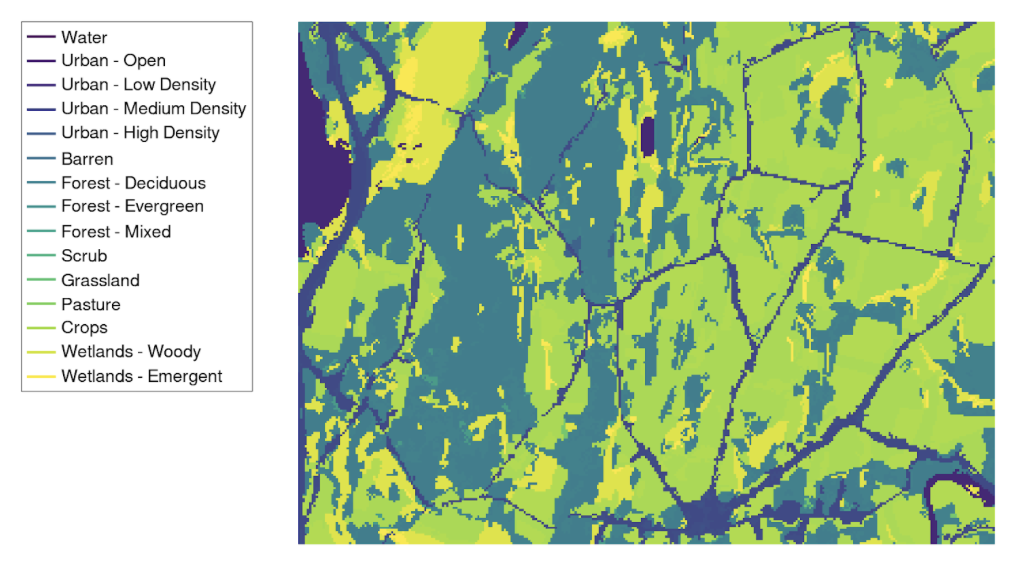
\includegraphics[width=.7\linewidth]{figure/lc5012}
    \caption{A plot of the NLCD data for the selected study area
    showing land-cover in real-year 2001, each 30m by 30m land cell is 
    colored based on its NLCD cover class (Table~\ref{tab:nlcd}),
    with similar colors being numerically closer classes.}
    \label{fig:land_plot}
\end{figure}

The land cells, as they exist in the NLCD data, provide the initial land
cover for the model within the starting year.
These land cells have been divided into land parcels,
which are the collections of cells that an agent in the model
has control over.
The properties that constitute the land cells within this model
are listed in Table~\ref{tab:land_cells},
and a diagram showing how this data is overlaid on the NLCD
data is shown in Figure~\ref{fig:land_cells}.

%% TAB: LAND_CELLS ---------------------------------------------------------
\begin{table}
\centering
\caption{Land Cell Features}
\label{tab:land_cells}
\begin{tabular}{llll}
\hline
\hline
    Parameter & Values \\
    \hline
    Parcel ID & Parcel that this cell is a part of \\
    Land Cover Category & Agricultural, Forested, Urban, Other \\
    NLCD Cover Class & See Table~\ref{tab:nlcd} \\
    Land Usage Type & Managed/In-Use, Adjacent, Unmanaged \\
    \hline
\end{tabular}
\end{table}

\begin{figure}
    \centering
    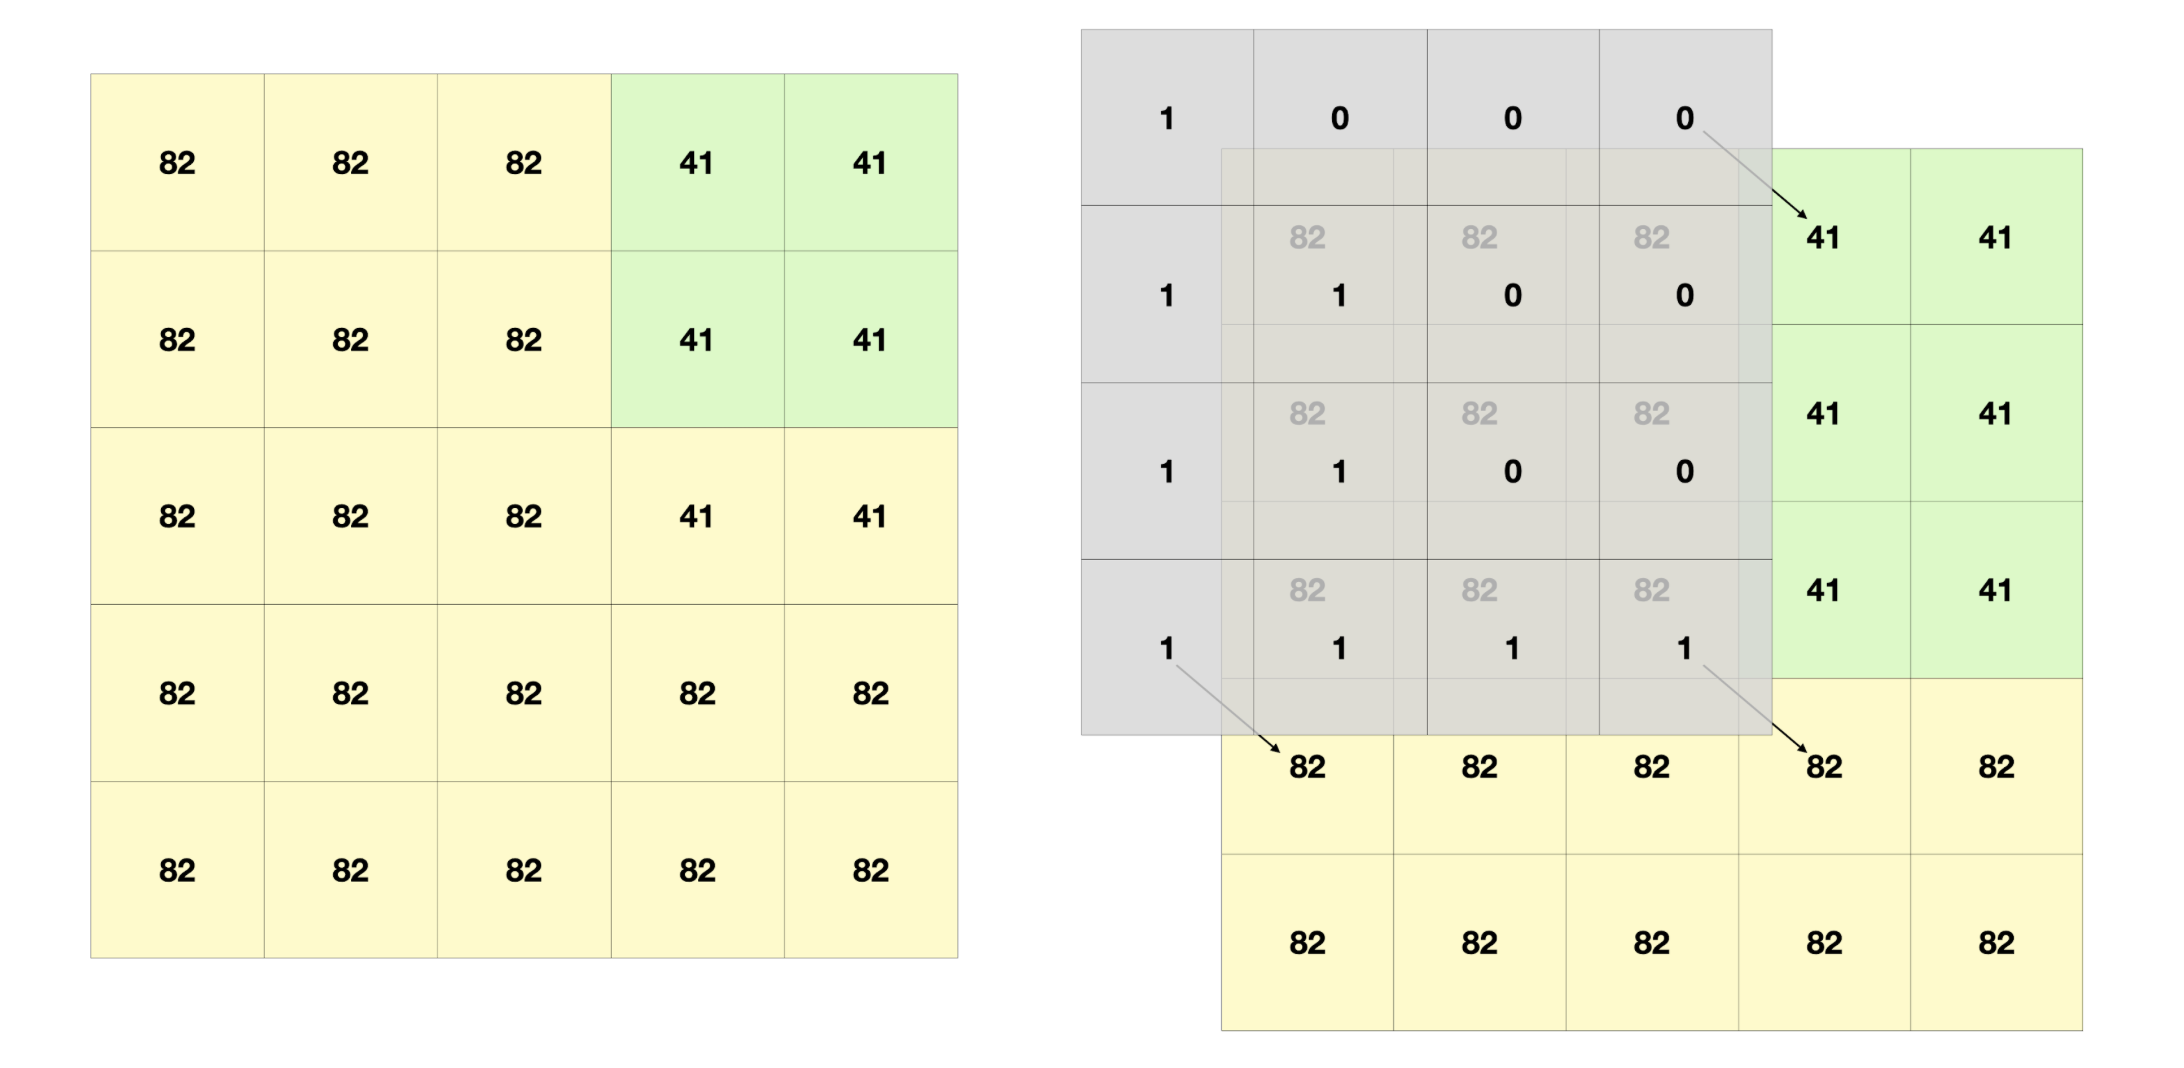
\includegraphics[width=0.7\textwidth]{figure/land-cells}
    \caption{Diagram showing how land cells and their
    associated properties are represented within the model as
    a grid of NLCD land cover values (left), and how those values
    have land use properties mapped onto them 1-1 (right).}
    \label{fig:land_cells}
\end{figure}

Initial land-use for the cells within the model is generated via
a stochastic process.
Within the land-use initialization, all cells start with
a label of ``unmanaged'',
then a number of cells within each parcel are labeled as ``managed'',
depending on the agent type and weighted towards population centers.
Finally, all cells which are ``unmanaged'' and border a ``managed''
cell are labeled as ``adjacent''.

\subsubsection{Agents}
\label{subsubsec:land_exp_agents}

There are four types of agent present in this model:
agricultural agents, forestry agents, commercial agents,
and residential agents.
There is one agent assigned for each land-parcel in the model,
and the agent type is assigned based on the majority land-cover
of the parcel.

Agricultural agents model the behavior of farmers, herders, 
and other kinds of agricultural land managers within the study area.
They make annual decisions about their farming practices,
including whether they should change production in one of the four modeled 
agricultural industries (beef, dairy, corn, and hay) 
and whether they should implement an agricultural best management practice 
(BMP) to reduce phosphorous runoff on their land.
This agent type has a very similar implementation in this model
as was described for the agricultural model in Section~\ref{sec:farm_ex},
but with the land-cover change further broken down by land-use.
It's modified state factors are listed in Table~\ref{tab:land_farmer_state},
and the actions it can take are listed in Table~\ref{tab:land_farmer_act}.

\begin{longtable}{lcll}
    \caption
    {A summary of the state factors being used during decision-making
    for agricultural agents in the land-cover model.} 
    \label{tab:land_farmer_state}
    \\
    \hline\hline
    Group && Description & Detail \\
    \hline
    \endfirsthead
    \caption[]{(continued...)} \\ \hline\hline
    Group && Description & Detail \\
    \hline
    \endhead
    \hline
    \endfoot
    Land Cover &$c_{c,m}$& Cropland/In-use & Cell Count \\
    &$c_{c,a}$& Cropland/Adjacent & Cell Count \\
    &$c_{p,m}$& Pasture/In-use & Cell Count \\
    &$c_{p,a}$& Pasture/Adjacent & Cell Count \\
    &$c_{a,u}$& Agricultural/Unmaintained & Cell Count \\
    &$c_{o,a}$& Other/Adjacent & Cell Count \\
    Productivity & $p_c$ & Corn & \\
    & $p_h$ & Hay & \\
    & $p_d$ & Dairy & \\
    & $p_b$ & Beef & \\
    History && BMP Adoption Record & \\
     && Extreme Event Record & \\
     && Net Profits/Losses & \\
    Network Information && BMP Adoption & \\
     && Net Profits/Losses & \\
\end{longtable}

In order to prevent any direct interference with the production functions,
an additional land-use decision action was added to the list of actions
for the agricultural agent, to explicitly capture the intent to change
the scope of land-use.
This action had initially been planned for inclusion in the agricultural
model described in Chapter~\ref{chap:farm}, but the lack of real-world
land-cover data in the associated datasets prevented its implementation.

\begin{longtable}{lp{0.5\textwidth}}
\caption{A summary of the action factors being used to drive agent
    decision-making for agricultural agents in the land-cover model.}
    \label{tab:land_farmer_act}\\
\hline\hline
Group & Action  \\
\hline\endfirsthead
\caption[]{(continued...)}\\
\hline\hline
Group & Action  \\
\hline\endhead
\hline\endfoot
BMP Usage & Adopt BMP  \\
    & Don't Adopt BMP  \\
Corn Production & Increase by $[0, S^+_c)$  \\
    & Maintain  \\
    & Decrease by $[0, S^-_c)$  \\
Hay Production & Increase by $[0, S^+_h)$  \\
    & Maintain \\
    & Decrease by $[0, S^-_h)$  \\
Dairy Production & Increase by $[0, S^+_d)$  \\
    & Maintain  \\
    & Decrease by $[0, S^-_d)$  \\
Beef Production & Increase by $[0, S^+_b)$  \\
    & Maintain  \\
    & Decrease $[0, S^-_b)$  \\
Land-Use Decision & Grow \\
& Maintain \\
& Shrink \\
\end{longtable}

Here, it behaves as follows.
A decision to ``maintain'' land-use means that no land-use changes will
occur. A decision to ``grow'' land-use means that the agent will search
for up~to~2 land cells which are of land-use ``adjacent'' to convert into
land-use ``maintained'', and will adjust its land area calculations
to match. A decision to ``shrink'' land-use means that the agent will
attempt the opposite transition, converting up~to~2 land cells from
land-use ``maintained'' to land-use ``adjacent''.
In all other agent types, this behavior is implicit to the actions that
the agents take and their associated scoping.

\begin{figure}
\centering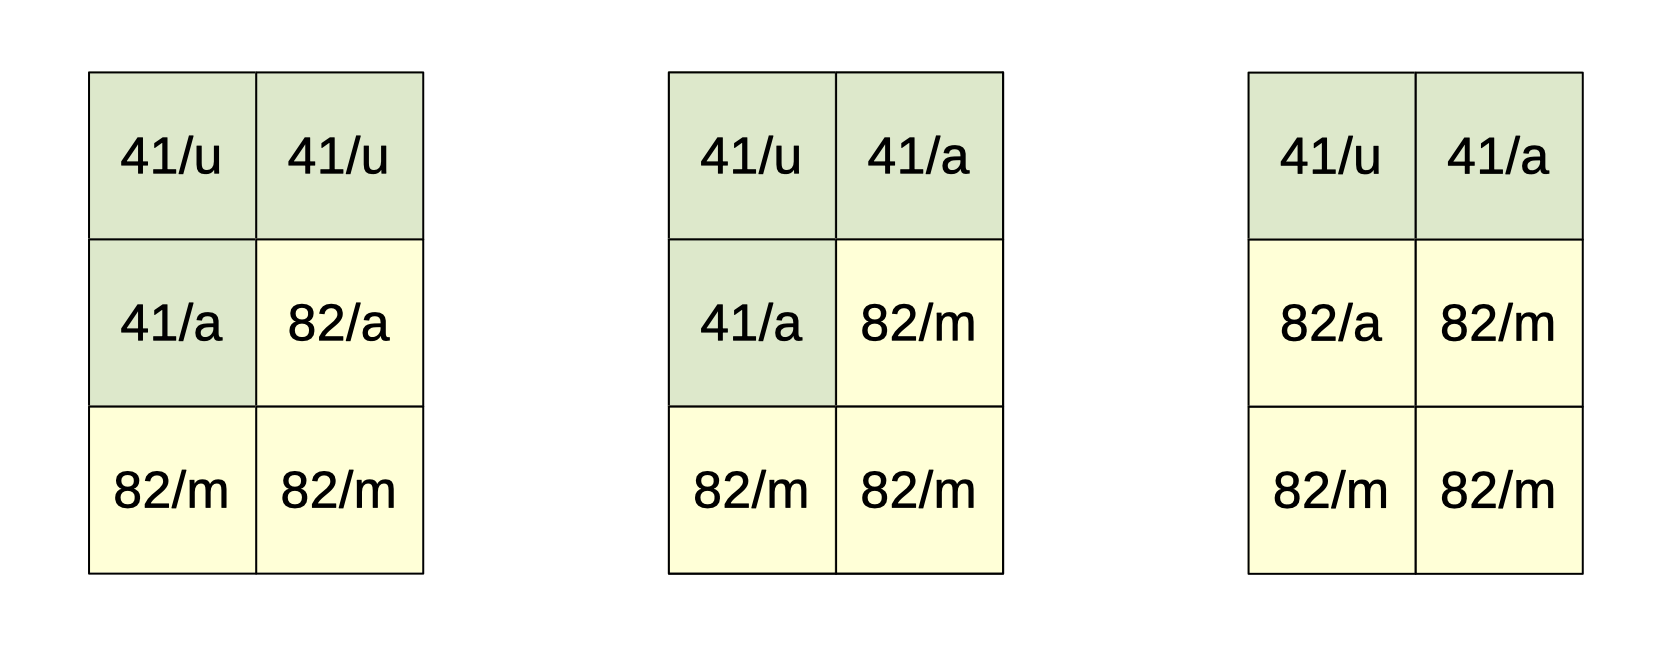
\includegraphics[width=0.7\textwidth]{figure/parcel-change}
\caption{Diagram showing how land-use, and consequently land-cover,
may change for an example 2-by-3 parcel over the course of a time-step.}
\end{figure}

Forestry agents model the behavior of loggers and other kinds of
forested land managers within the study area.
They make annual decisions about their practices
and whether to implement an advised management practice (AMP)
on their land.
The forestry agents are implemented very similarly to the
agricultural agents, but the land-cover of interest has been changed
to forested land, and the production function has been replaced with
a generalized forested productivity function.
The state factors used by the forestry agents in their decision-making
are listed in Table~\ref{tab:land_forest_state},
and the actions that these agents can take are listed
in Table~\ref{tab:land_forest_act}.

\begin{longtable}{lcll}
\caption{A summary of the state factors being used during decision-making
for forestry agents in the land-cover model.} 
\label{tab:land_forest_state}
\\
\hline\hline
Group && Description & Detail \\
\hline
\endfirsthead
\caption[]{(continued...)}
\\
\hline\hline
Group && Description & Detail \\
\hline
\endhead
\hline
\endfoot
Land Cover &$c_{f,m}$& Forested/In-use & Cell Count \\
&$c_{f,a}$& Forested/Adjacent & Cell Count \\
&$c_{f,u}$& Forested/Unmaintained & Cell Count \\
&$c_{o,a}$& Other/Adjacent & Cell Count \\
Productivity &$p_f$& Forestry & \\
History && AMP Adoption & \\
 && Extreme Event Record & \\
 && Net Profits/Losses & \\
Network Information && AMP Adoption & \\
 && Net Profits/Losses \\
\end{longtable}

\begin{longtable}{lp{0.5\textwidth}}
\caption{A summary of the action factors being used to drive agent
    decision-making for forestry agents in the land-cover model.}
\label{tab:land_forest_act} \\
\hline\hline
Group & Action   \\
\hline\endfirsthead
\hline\endfoot
AMP Usage & Adopt AMP  \\
    & Don't Adopt AMP  \\
Forestry Decision & Increase by $[0, S^+_f)$  \\
    & Maintain  \\
    & Decrease by $[0, S^-_f)$  \\
\end{longtable}

Agricultural and forestry agents are connected to and share information with
their 5-nearest neighbors of the same agent type; these
networks are static throughout each model run.
For both of these agent types, their learning reward is based on their
net profitability as was described in Chapter~\ref{chap:farm}.

Commercial agents model the behavior of shops, factories, offices, 
and other kinds of commercial land-holders within the study area. 
They make decisions bi/trimonthly about their workforce, 
including their available jobs and the associated salaries.
Byproducts of their actions impact the density and sprawl of urban
land cover on the landscape.
The state factors that it uses in decision-making are listed
in Table~\ref{tab:land_com_state},
and the actions they can take are listed
in Table~\ref{tab:land_com_act}.

\begin{longtable}{lp{0.5\textwidth}}
\caption{A summary of the state factors being used during decision-making
for commercial agents in the land-cover model.}
\label{tab:land_com_state}\\\hline\hline
Group & Description  \\\hline\endfirsthead
\hline\endfoot
Financial Status & \\
Employees & Capacity \\
    & Actual \\
    & Utilization \\
\end{longtable}

\begin{longtable}{lp{0.5\textwidth}}
\caption{A summary of the action factors being used to drive agent
    decision-making for commercial agents in the land-cover model.} 
    \label{tab:land_com_act}\\
\hline\hline
Group & Action  \\
\hline\endfirsthead
\caption[]{(continued...)}\\
\hline\hline
Group & Action \\
\hline\endhead
\hline\endfoot
Business Capacity & Decrease  \\
& Maintain  \\
& Increase  \\
Employees & Fire  \\
& Maintain  \\
& Hire  \\
\end{longtable}

Commercial agents use a simple compound reward function for their
performance, with a `living reward'~$t_l$, which grows as the number of 
time steps the commercial agent has gone without declaring bankruptcy
/ employee count becoming zero,
and the realized utilization~$U_e$ of their land,
such that the reward~$R_c=t_l*U_e$.

Residential agents model the behavior of renters and landowners within 
the study area. 
They make two decisions annually: whether to attempt a job change 
and whether to try to move houses. 
Household satisfaction, and their reward value~$R_r$,
is valued as a combination of financial stability 
and mental satisfaction. 
Each household earns wages provided by a commercial agent --- 
these wages are determined by a stochastic process and can be adjusted by 
the job over time.
The decisions of these agents do not directly impact land cover change
on their associated parcel, but land cover can transition within their
parcel as a result of the decisions of other agents.

\begin{longtable}{lp{0.5\textwidth}}
\caption{A summary of the state factors being used during decision-making
for residential agents in the land-cover model.}
\label{tab:land_res_state} \\ \hline \hline
Group & Description \\ \hline \endfirsthead
\hline \endfoot
Financial Status & \\
Length in State & \\
Household Budget & Monthly \\
Household Budget & Yearly \\
Failed Action Count & Consecutive \\
\end{longtable}

\begin{longtable}{lp{0.5\textwidth}}
\caption{A summary of the action factors being used to drive agent
    decision-making for residential agents in the land-cover model.} \\
\hline\hline
Group & Action  \\
\hline\endfirsthead
\caption[]{(continued...)} \\
\hline\hline
Group & Action  \\
\hline\endhead
\hline\endfoot
Employment & Search for new job  \\
 & Keep current job  \\
Housing & Search for new housing  \\
& Keep same housing \\
\end{longtable}

The reward function used by residential agents is similar
to that used by commercial agents, but the living reward is
scaled by the agent's financial status.

Commercial and residential agents exist in a bipartite network with
one another.
This network is initialized via a stochastic process and is
updated as agents make decisions.
This process is detailed in Appendix~\ref{app:land},
alongside other details of agent initialization.

The learning architecture for agents of each type is
listed in Table~\ref{tab:land_anns}.
Similarly to the agent-networks described in the
model in Chapter~\ref{chap:farm},
all networks are fully-connected,
use ReLU activation and He Initialization,
and use $n$-hot output to encode their selected action.
Additionally, all target architectures are initially identical
to the active network architectures as specified below.

\begin{table}[h]
\centering
\caption{Network parameters for the ANNs used by agents in each class
    for the land cover model}
\label{tab:land_anns}
    \begin{tabular}{@{\extracolsep{4pt}}lp{.05\linewidth}>{\centering}p{.05\linewidth}>{\centering}p{.05\linewidth}>{\centering}p{.05\linewidth}>{\centering}p{.05\linewidth}>{\centering}p{.05\linewidth}>{\centering}p{.05\linewidth}cc@{}}
\hline
\hline
\multirow{2}{*}{Parameter} 
    & \multicolumn{2}{c}{Agricultural} & \multicolumn{2}{c}{Forestry} 
    & \multicolumn{2}{c}{Commercial} & \multicolumn{2}{c}{Residential} \\
    \cline{2-3}\cline{4-5}\cline{6-7}\cline{8-9}
 & $\mu$ & $Q$ & $\mu$ & $Q$ & $\mu$ & $Q$ & $\mu$ & $Q$  \\
\hline
Input Nodes  & 15 & 32 & 10 & 15 & 4 & 10 & 5 & 9 \\
Inner Layers  & 4 & 3 & 4 & 3 & 2 & 2 & 2 & 2 \\
Inner Nodes  & 10 & 16 & 7 & 7 & 5 & 5 & 4 & 5 \\
Output Nodes  & 17 & 1 & 5 & 1 & 6 & 1 & 4 & 1 \\
\hline
\end{tabular}
\end{table}

\subsubsection{Model Hyperparameters}

A summary of the fixed hyperparameters across all runs of this
model are listed in Table~\ref{tab:land_hyper}.
Many of the parameters are taken directly from the
agricultural model described in Chapter~\ref{chap:farm},
with the economic production functions taking from the
corresponding model years and the weather generation
submodel using the baseline case of $\Delta EE = 0$.

The length of the training episode was set to 60 time-steps,
or 5 model-years, to match the granularity of the real-world
NLCD~datasets.
Preliminary model runs for determining appropriate fixed
model hyperparameters were done with the land-cover data
from NLCD year 2001 as input data, comparing
the data from NLCD year 2006 with the model output year 2006.

\begin{longtable}{lcll}
\caption{Fixed hyperparameters and their associated values
for the land-cover change model.}
\label{tab:land_hyper}\\\hline\hline
Parameter & & Value \\
\hline\endfirsthead
\caption[]{(continued...)}\\\hline\hline
Parameter & & Value \\
\hline\endhead
\hline\endfoot
Learning Rate & $\alpha$ & 0.00025 \\
Exploration Rate & $\epsilon$ & 0.1 \\
Base Transfer Rate & $\tau$ & 0.001 \\
Transition Memory Size & $M$ & 10000 \\
Number of Steps per Episode & $T$ & 60 \\
\end{longtable}

\subsubsection{Evaluating Model Performance}

For this model, the Nash-Sutcliffe efficiency index (NSE) was used
to evaluate the goodness-of-fit of model output at the end of each
training episode.
The NSE is a measure of the relative magnitude of the residual variance of
modeled data compared to the residual variance of the observed data.
The value of the index ranges from~$-\infty$~to~1,
where a score of 1 indicates a perfect fit,
a score of 0 indicates that the model's fit is no better than the mean
of the observed data,
and a score less than 0 indicates that the mean of the observed data
is a better predictor than the model.

This index was calculated in relation to three forms of model performance.
The first is the ability of the model to appropriately predict
the proportional coverage of each land cover type in the target year,
$\text{NSE}_\text{plc}$.
The second is the ability of the model to appropriately predict
the categorical transitions of land cover types from the start year to
the target year,
$\text{NSE}_\text{cat}$.
The third is the ability of the model to appropriately predict
the absolute transitions of land cover types from the start year to
the target year,
$\text{NSE}_\text{abs}$.
These indices are detailed below.

A majority of land cells in the study area do not transition land cover
between the start year and target year ($92.6\%, n=69124$),
which would heavily bias any analysis of model performance.
Therefore, these NSE indices were only calculated for those cells
that transitioned land cover.

The NSE measure of proportional coverage ($\text{NSE}_\text{plc}$)
is shown in Equation~\ref{eq:nse_plc},
where~$P_B$ represents the observed proportional coverage of land cover
category~$B$ in the target year,
$\hat{P_B}$~represents the simulated proportional coverage of land cover
category~$B$ in the target year,
and~$\bar{P_B}$ represents the mean observed proportional coverage of
land cover category~$B$ in the target year.

\begin{equation}
    \label{eq:nse_plc}
    \text{NSE}_{\text{plc}} 
    = \frac{\sum_B\left(P_B - \hat{P_B}\right)^2}
        {\sum_B\left(P_B-\bar{P_B}\right)^2}
\end{equation}

The NSE measure of categorical land cover transitions 
($\text{NSE}_\text{cat}$), shown in Equation~\ref{eq:nse_cat},
where $\Delta_{A,B}$ represents the number of observed transitions
from land cover category $A$ in the starting year to land cover
category $B$ in the target year,
for the overarching categories shown in Table~\ref{tab:nlcd},
where $\widehat{\Delta_{A,B}}$ represents 
the number of simulated transitions from $A$ to $B$,
and where $\overline{\Delta_{A,B}}$ represents the mean observed number of
transitions from $A$ to $B$.

\begin{equation}
    \label{eq:nse_cat}
    \text{NSE}_{\text{cat}}
    = \frac{\sum_{A,B}\left(\Delta_{A,B}-\widehat{\Delta_{A,B}}\right)^2}
        {\sum_{A,B}\left(\Delta_{A,B}-\overline{\Delta_{A,B}}\right)^2},
    A \ne B
\end{equation}

The NSE measure for absolute land cover transition 
($\text{NSE}_\text{act}$), shown in Equation~\ref{eq:nse_act},
is very similar to the calculation of $\text{NSE}_\text{cat}$,
except that it is calculated for the absolute land cover class of each
land cell and not just its categorical class.
This index is a stricter metric than the previous two indices,
as, for example,
a modeled transition from cropland to deciduous forest $\delta_{82,41}$
compared to an observed transition to mixed forest $\delta_{82,43}$,
which would be labeled ``correct'' according to $\NSE{cat}$
would be considered a misclassification according to $\NSE{abs}$.

\begin{equation}
    \label{eq:nse_act}
    \text{NSE}_{\text{abs}} 
    =
    \frac{\sum_{a,b}\left(\Delta_{a,b} - \widehat{\Delta_{a,b}}\right)^2}
        {\sum_{a,b}\left(\Delta_{a,b} - \overline{\Delta_{a,b}}\right)^2}
    ,
    a\ne b
\end{equation}

For the purposes of model calibration,
as described in Section~\ref{sec:land_cal},
the model was calibrated to maximize the result of $\NSE{cat}$
for the transition from the starting year 2006,
to the observed and modeled year 2011.

\subsubsection{Execution Overview}

A high-level overview of model execution,
showing the main training loop with the transfer calibration step
and the final testing loop, is shown 
in Figure~\ref{fig:land_exec_training}.
A more-detailed overview of model execution, specifically focused on
the behavior and training and agents is
shown in Figure~\ref{fig:land_exec_2}.

\begin{figure}
\centering
    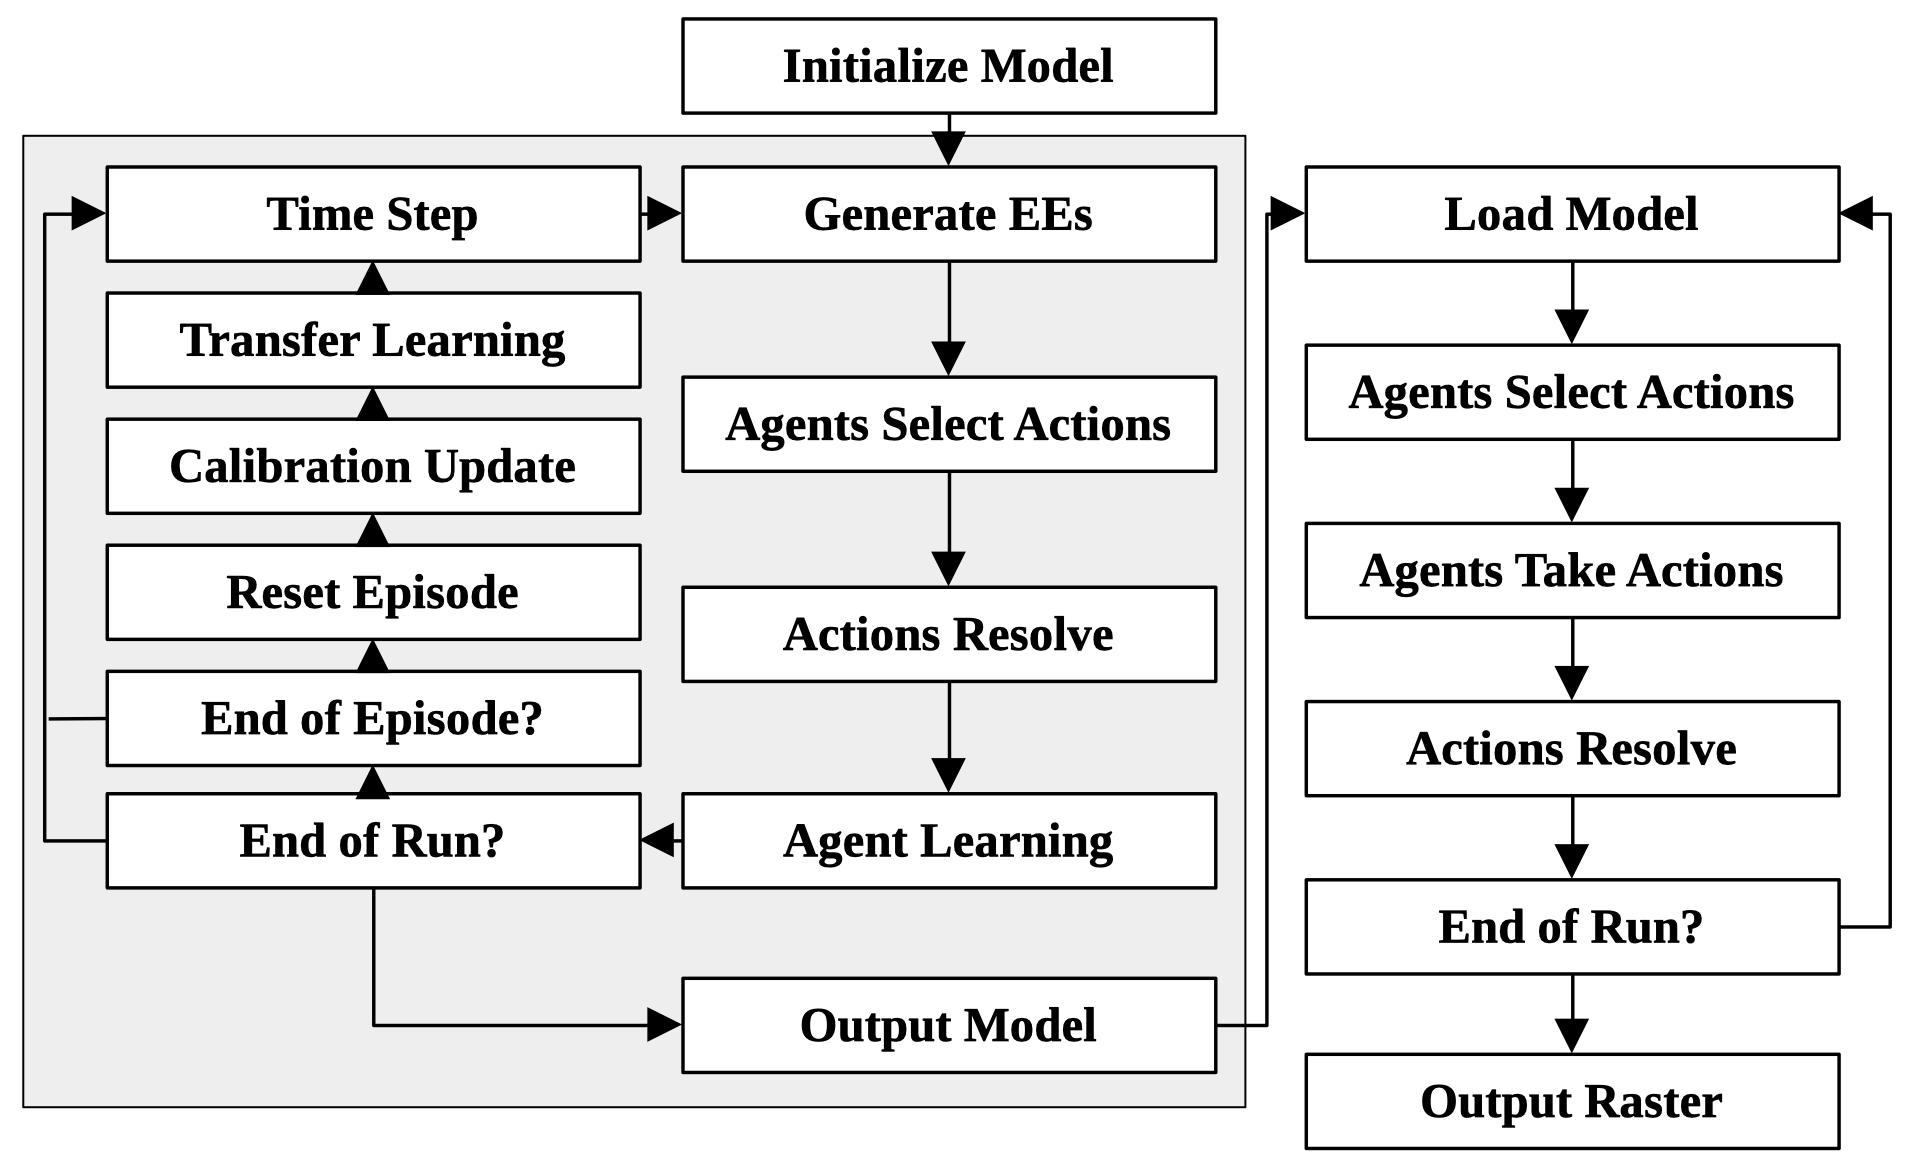
\includegraphics[width=0.7\linewidth]{figure/land-flow}
    \caption{Flowchart showing a high-level overview of model
    execution between the main training/calibration loop (left),
    and the final testing runtime loop (right)}
    \label{fig:land_exec_training}
\end{figure}

\begin{figure}
\centering
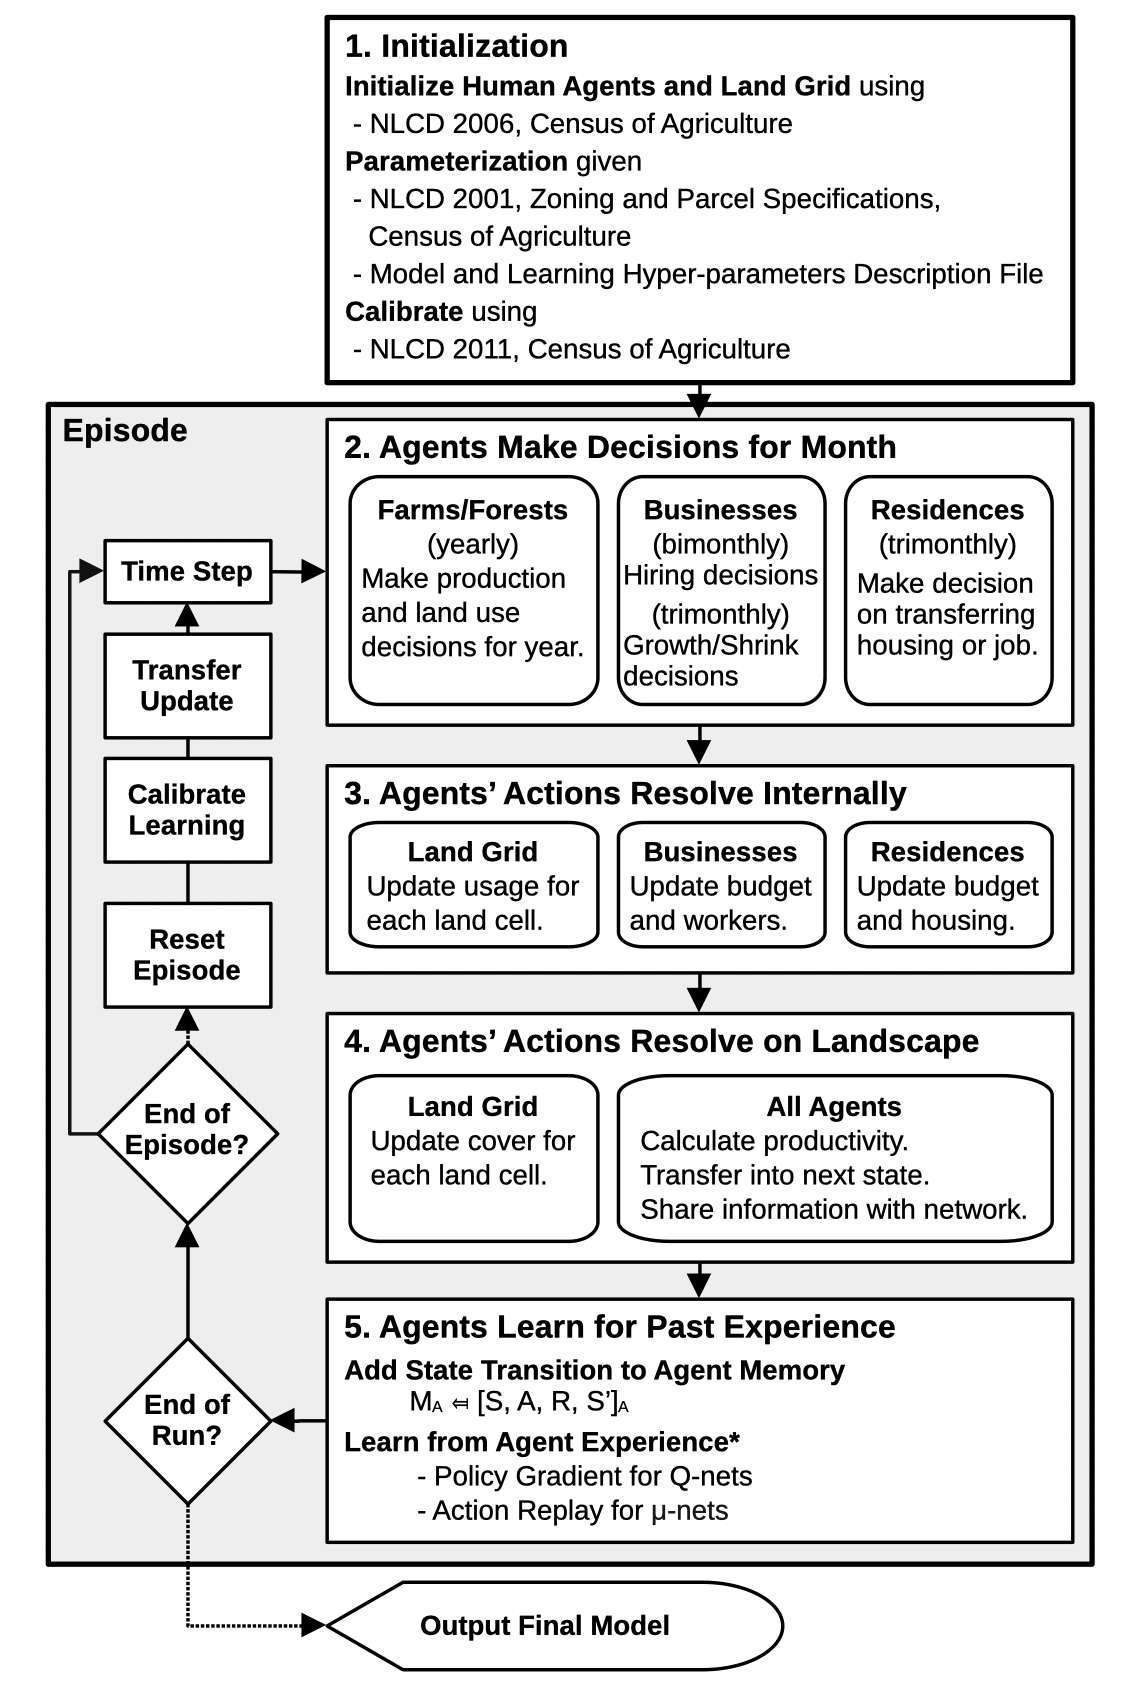
\includegraphics[width=0.7\textwidth]{figure/flowchart2.png}
\caption{Flowchart demonstrating the overall execution of the agent-based model
    and its coupling with the machine learning processes}
\label{fig:land_exec_2}
\end{figure}

%%%%%%%%%%%%%%%%%%%%%%%%%%%%%%%%%%%%%%%%%%%%%%%%%%%%%%%%%%%%%%%%%%%%%%%%%%%
%%%%%%%%%%%%%%%%%%%%%%%%%%%%%%%%%%%%%%%%%%%%%%%%%%%%%%%%%%%%%%%%%%%%%%%%%%%

\subsection{Experimental Setup}
\label{subsec:land_exp_setup}

In order to avoid some of the high levels of variance seen
in the experimental runs of the agricultural model and that model's sensitivity
to agent paramterization, these experimental runs were limited in scope
to a subset of model hyperparameters that relate to agent memory
and foresight, listed in Table~\ref{tab:land_exp}.
Each combination of parameterizations was tested for 40 model runs.

Replay batch size~$B$ was tested for the sizes 8, 16, 32, and~64.
This value determines how many state transition records are sampled
during the action-replay and policy gradient learning steps.
A higher number of records sampled increases the smoothness of
the gradient being sampled, at the cost of extra computation.

The discount factor~$\gamma$ was tested for the values $0.5, 0.9$,
and $0.99$.
This factor is used in the Q-learning update (Eq~\ref{eq:q_update})
to discount the expected rewards at a future time-step.
A lower value of~$\gamma$ indicates a lower value of the
reward in step $t+1$ than the current reward in step $t$,
which compounds multiplicably with each additional time-step forward.

The recall accuracy~$F'$, is the notational inverse of the
forgetfulness factor described in Section~\ref{subsec:farm_methods_memory},
where $F'=(1-F)$ and consequently a recall accuracy of~1 indicates agents
with~0 forgetfulness, that is, perfect record recall.

\begin{table}
\caption{Experimental parameters that were tested in experimental runs
of the land-cover transition model}
\label{tab:land_exp}
\centering
\begin{tabular}{lcl}
\hline
\hline
    Variable && Values \\
    \hline
    Batch Size & $B$ & 8, 16, 32, 64 \\
    Discount Factor & $\gamma$ & 0.5, 0.9, 0.99 \\
    Recall Accuracy & $F'$ & 0, 0.25, 0.5, 0.75, 1 \\
    \hline
\end{tabular}
\end{table}

% For the purposes of analyzing the results of this model,
% where these types of transitions occur,
% they are treated as neither a successful nor an unsuccessful measure
% of model performance.
% Instead, they are treated as a separate neutral measure.
% 
% This limitation of the model is discussed in greater detail
% in Section~\ref{sec:land_disc}.
% 
% 
% For many of these missing transitions,
% there is a lack of any substantive literature supporting a predictive model 
% that is generalizable enough to meaningfully incorporate into the ABM.


\section{Results}
\label{sec:land_results}

\subsection{Model Performance}
\label{subsec:land_results_performance}

Model performance under each experimental parameterization was
evaluated by comparing the land cover in model year 2016 to
the recorded/observed land cover for the study area for real year 2016.

The maximum NSE values seen during testing runs were 
$\text{NSE}_\text{plc} = 0.84$,
$\text{NSE}_\text{cat} = 0.76$, and
$\text{NSE}_\text{act} = 0.64$.
The sensitivity of these indices to each of the experimental parameters
was evaluated by calculated the mean and variance of the indices
under each parameterization across all 40 runs.
These results have been plotted in Figure~\ref{fig:land_nse}.

\begin{figure}
    \centering
    \subcaptionbox{$\text{NSE}_\text{plc}$}{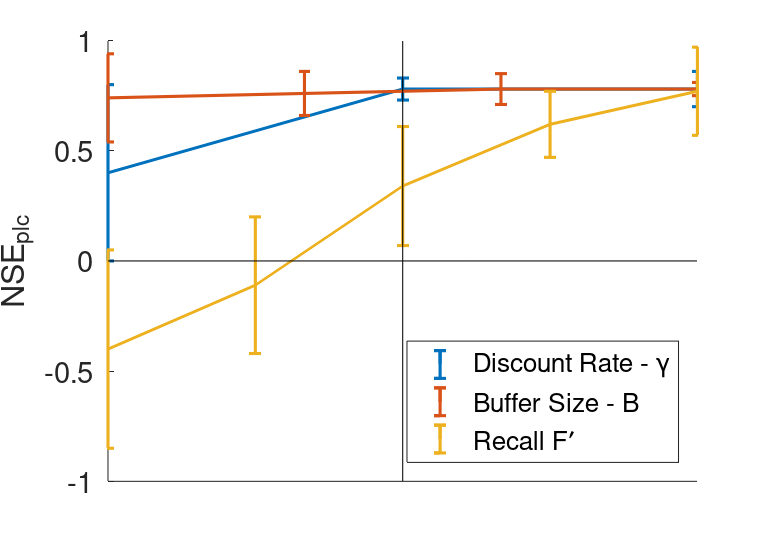
\includegraphics[width=0.3\textwidth]{figure/nscplc}}
    \hfill
    \subcaptionbox{$\text{NSE}_\text{cat}$}{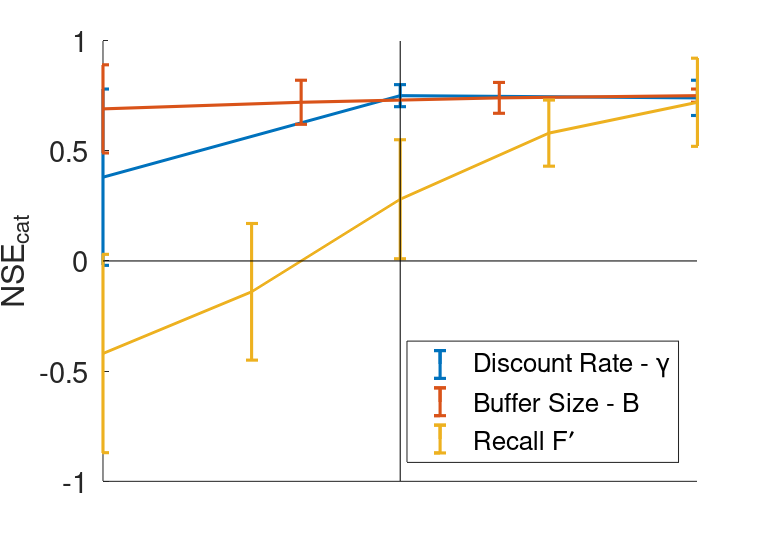
\includegraphics[width=0.3\textwidth]{figure/nsccat}}
    \hfill
    \subcaptionbox{$\text{NSE}_\text{act}$}{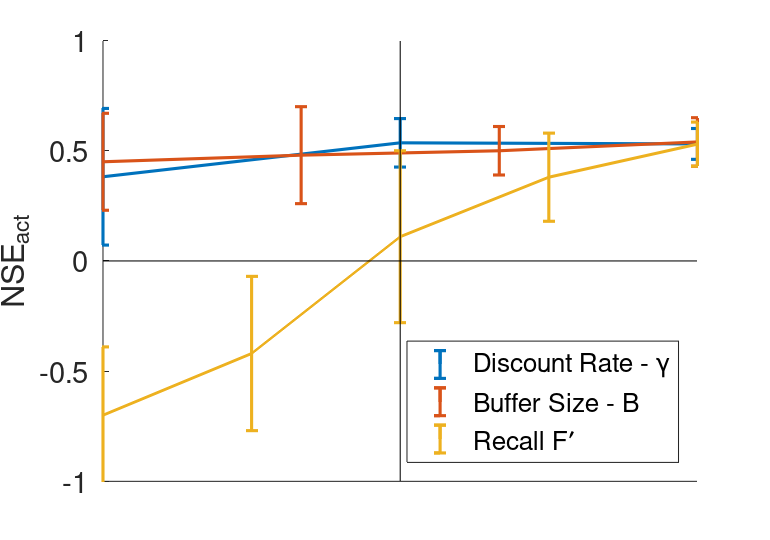
\includegraphics[width=0.3\textwidth]{figure/nscact}}
    \caption{NSE index sensitivity for each index showing the variance in
    model classification accuracy by each metric under different model
    parameterizations.}
    \label{fig:land_nse}
\end{figure}

In order to better understand the output of the model and where misclassification was
occurring within testing runs, the land-cover transition matrices were analyzed.
Categorical cover change had been used as the calibration function for the model,
so land cover transitions were divided into three primary categories: urban~$U$,
forested~$F$, and agricultural~$A$, and an other~$O$ category for all other land-cover categories;
and instances where both the real and modeled data
had a matching transition from a land-cover category to itself were removed.

For the purposes of this discussion,
the two land-cover transition matrices that will be compared against the actual
land-cover transition are the ``best fit'' model ($\NSE{cat}=0.76$)
and the ``best median'' model, the median performer for the 
highest scoring parameterization during testing ($\NSE{cat}=0.68$, $\gamma=0.99$, $B=64$, $F'=1$).
Arrow plots, summarizing how land-cover transitions compared between these models,
are shown in Figure~\ref{fig:arrows},
with the associated confusion matrices listed in Table~\ref{tab:confusion}

\begin{figure}
\centering
\subcaptionbox{Observed Cover Change}{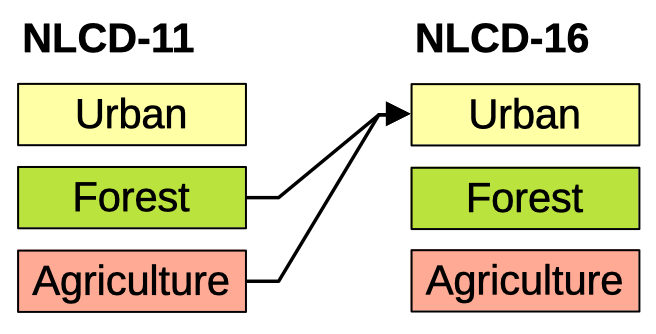
\includegraphics[width=0.3\textwidth]{figure/cat_obs}}
\hfill
\subcaptionbox{``Best Fit'' Cover Change}{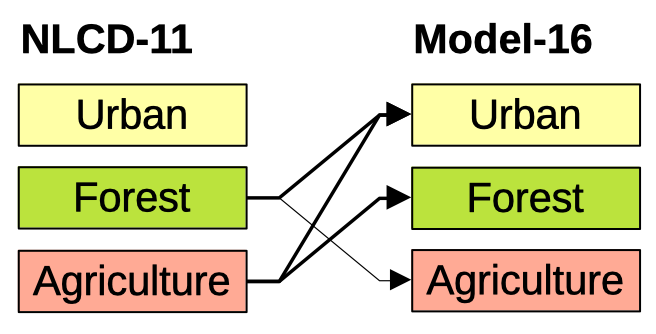
\includegraphics[width=0.3\textwidth]{figure/cat_max}}
\hfill
\subcaptionbox{Best Median Change}{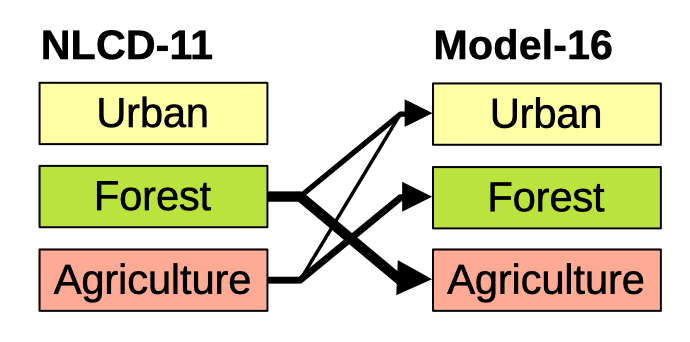
\includegraphics[width=0.3\textwidth]{figure/cat_med}}
\caption{Arrow plots showing a comparison of the categorical transitions between
the three main land-cover categories between
(a) the real world data, and (b) the ``best-fit'' model, and (c) the ``best median'' model.
Arrow width between NLCD-11 and 2016 is proportional to the number of transitions between the
connected categories.}
\label{fig:arrows}
\end{figure}

\begin{table}
    \centering
    \caption{Confusion matrix comparing the resulting categorical transitions from the NLCD data to the modeled transitions
    for both the best fit, and best performing parameterization.
    Because the initial cover category for both transitions are definitionally equal,
    it has been omitted from the header row.
    The transition $\Delta_{*,O}$ represents a transition outside one of the three major cover categories.}
    \label{tab:confusion}
    \begin{tabular}{@{\extracolsep{4pt}}c|cccc|cccc@{}}
    & \multicolumn{4}{c}{``Best Fit'' 2016} & \multicolumn{4}{c}{Best Median 2016} \\ \cline{2-5}\cline{6-9}
    NLCD 2016 & $\Delta_{*,U}$ & $\Delta_{*,F}$ & $\Delta_{*,A}$ & $\Delta_{*,O}$ 
    & $\Delta_{*,U}$ & $\Delta_{*,F}$ & $\Delta_{*,A}$ & $\Delta_{*,O}$ \\ \hline
    $\Delta_{U,U}$ & --- & 0 & 0 & 0 & --- & 0 & 0 & 0 \\
    $\Delta_{U,F}$ & 0 & 0 & 0 & 0 & 0 & 0 & 0 & 0 \\
    $\Delta_{U,A}$ & 0 & 0 & 0 & 0 & 0 & 0 & 0 & 0 \\
    $\Delta_{U,O}$ & 0 & 0 & 0 & 0 & 0 & 0 & 0 & 0 \\ \hline
    $\Delta_{F,U}$ & 7 & 0 & 0 & 0 & 7 & 0 & 0 & 0 \\
    $\Delta_{F,F}$ & 1 & --- & 5 & 0 & 0 & --- & 7 & 0 \\
    $\Delta_{F,A}$ & 0 & 0 & 0 & 0 & 0 & 0 & 0 & 0\\
    $\Delta_{F,O}$ & 0 & 7 & 0 & 36 & 3 & 5 & 5 & 30 \\ \hline
    $\Delta_{A,U}$ & 11 & 0 & 0 & 0 & 11 & 0 & 0 & 0 \\
    $\Delta_{A,F}$ & 0 & 0 & 0 & 0 & 0 & 0 & 0 & 0 \\
    $\Delta_{A,A}$ & 7 & 1 & --- & 0 & 3 & 14 & --- & 0 \\
    $\Delta_{A,O}$ & 0 & 4 & 4 & 3  & 1 & 0 & 10 & 0 \\
    \end{tabular}
\end{table}

Within the study area, cells with urban land-cover did not transition into any 
other category of land-cover during the study period.
Forested and agricultural cells which did transition categories,
primarily developed into urban land-cover, followed by
transitions into other categorizations.
These forested and agricultural transitions are the primary source of
the classification error within these models and are discussed further
is the following section.

\section{Discussion}
\label{sec:land_disc}

The experimental parameters which were tested each had a different degree
of impact on model performance.
The recall factor~$F'$, had the strongest impact on model performance,
with values less than 0.75 resulting in model runs that were worse performers
than the probabilistic average for $\NSE{act}$,
and with a value of 0.5 resulting in worse performance than average for
all 3~indices.
In the case of $\NSE{act}$, there is a noticeable drop in model performance
for the case of $\gamma=0.99$ compared to $\gamma=0.9$; however, 
this change is not large enough to be statistically significant when
the variance in model performance for the case of $\gamma=0.9$ is considered.

Looking at the transition plots and confusion matrices for some of the
higher accuracy model runs,
the largest source of error within the tested models came from land-cover
transitions between the agricultural and forested land-cover categories.
These transitions, like most land cover transitions between cover categories,
were poorly represented within the calibration data, as land-cover transition
is a relatively slow process that even the 5-year interval of the NLCD dataset
has difficulty capturing.
Similarly, the highest performing models tended to overclassify urbanization land-cover
changes, which were the most represented cross-category land-cover change 
in the calibration data set.

The categorical classification into the group other~$O$ was the most accurate cross-category
predictor --- in particular, categorical transition into the Grassland/Scrub cover-category.
These transitions are present in the calibration and testing datasets,
and frequently occur in proximity to changes in agricultural and forested land-cover changes.
It is possible that this is related to the high confusion in the land-cover transitions
between agricultural and forested land-cover regions, but that level of testing would
require land-cover datasets for similar regions with similar land-cover transition patterns,
which were outside of the scope of this modeling effort.

If this work were to be continued, it would be interesting to see how this type of
integrated land-cover transition model would perform over a longer period of time
or wihtin a larger study area, so the number of and type of land-cover transitions
occurring within the calibration dataset would be more representative of the
land-cover transitions occurring within the study period.
